

\begin{figure}[t] 
\centering
\newcommand\morphwidth{.9}
\subfloat{
    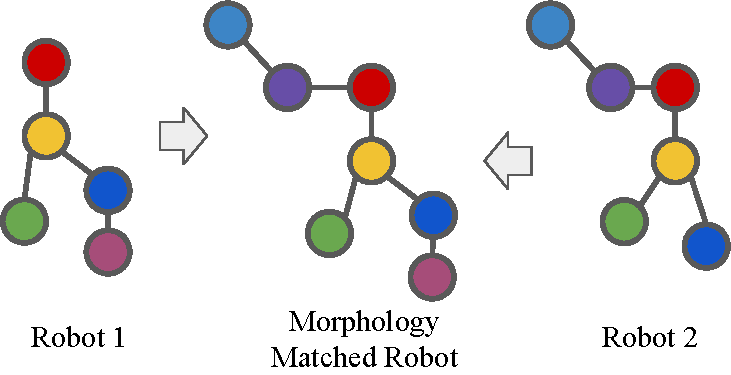
\includegraphics[width=\morphwidth\linewidth, valign=t]{Figures/morphology_matching.pdf}
}
\caption{ \textbf{Morphology matching of two robots.}
Though the two robots may be different in morphology (i.e. kinematic tree topology), by properly choosing a root node (e.g. the yellow node), we can always add new nodes and edges to the kinematic tree of the robot(s) to match their morphology.
}
\label{fig:morph}
\end{figure}

